\documentclass{beamer}

\usepackage[hashEnumerators,smartEllipses]{markdown}
\usepackage{pgfplots, pgfplotstable}
\usepackage{booktabs}
\usepackage{scalerel}
\usepackage{framed} 
\usepackage{tikz}
\usepackage{natbib}
\usepackage{float}
\usepackage{etoolbox}
\usepackage{caption}
\usepackage{subcaption}
\usepackage{listings}
\usepackage{lstautogobble}
\usepackage{xcolor}
\usepackage{tikz}
%\usepackage{pgf-pie}
\usetikzlibrary{decorations.pathreplacing,calc,shapes,positioning,tikzmark, trees}
\pgfplotsset{compat=1.17}

%\setlength\parindent{0pt}

\definecolor{darksky}{rgb}{0.4,0.4,1}
\definecolor{skyblue}{rgb}{0.25,0.78,0.96}
\definecolor{lightyellow}{rgb}{1,0.96,0.52}
\definecolor{lightorange}{rgb}{1,0.7,0.4}
\definecolor{lightred}{rgb}{1,0.4,0.4}

\definecolor{codegreen}{rgb}{0,0.6,0}
\definecolor{codegray}{rgb}{0.5,0.5,0.5}
\definecolor{codepurple}{rgb}{0.58,0,0.82}
\definecolor{backcolour}{rgb}{0.95,0.95,0.92}

\lstdefinestyle{python}{
    backgroundcolor=\color{backcolour},   
    commentstyle=\color{codegreen},
    keywordstyle=\color{magenta},
    numberstyle=\tiny\color{codegray},
    stringstyle=\color{codepurple},
    basicstyle=\ttfamily\footnotesize,
    breakatwhitespace=false,         
    belowskip=-0.5em,
    breaklines=true,                 
    captionpos=b,                    
    keepspaces=true,                 
    numbers=true,                    
    numbersep=5pt,                  
    showspaces=false,                
    showstringspaces=false,
    showtabs=false,                  
    tabsize=4
}

\lstset{style=python}

\usetikzlibrary{arrows}

%
%
%


\definecolor{rosso}{RGB}{220,57,18}
\definecolor{giallo}{RGB}{255,153,0}
\definecolor{blu}{RGB}{102,140,217}
\definecolor{verde}{RGB}{16,150,24}
\definecolor{viola}{RGB}{153,0,153}


\tikzset{
    chart/.style={
        legend label/.style={font={\scriptsize},anchor=west,align=left},
        legend box/.style={rectangle, draw, minimum size=5pt},
        axis/.style={black,semithick,->},
        axis label/.style={anchor=east,font={\tiny}},
    },
    pie chart/.style={
        chart,
        slice/.style={line cap=round, line join=round, very thick,draw=white},
        pie title/.style={font={\bfseries}},
        slice type/.style 2 args={
            ##1/.style={fill=##2},
            values of ##1/.style={}
        }
    }
}

\pgfdeclarelayer{background}
\pgfdeclarelayer{foreground}
\pgfsetlayers{background,main,foreground}


\newcommand{\pie}[3][]{
    \begin{scope}[#1]
        \pgfmathsetmacro{\curA}{90}
        \pgfmathsetmacro{\radius}{1}
        \def\Centre{(0,0)}
        \node[pie title] at (90:1.3) {#2};
        \foreach \v/\s in{#3}{
            \pgfmathsetmacro{\deltaA}{\v/100*360}
            \pgfmathsetmacro{\nextA}{\curA + \deltaA}
            \pgfmathsetmacro{\midA}{(\curA+\nextA)/2}

            \path[slice,\s] \Centre
            -- +(\curA:\radius)
            arc (\curA:\nextA:\radius)
            -- cycle;

            % to determine direction of lines (left/right, up/down
            \pgfmathsetmacro{\ysign}{ifthenelse(mod(\midA,360)<=180,1,-1)}
            \pgfmathsetmacro{\xsign}{ifthenelse(mod(\midA-90,360)<=180,-1,1)}

            \begin{pgfonlayer}{foreground}
                \draw[*-,thin] \Centre ++(\midA:\radius/1.5) -- 
                ++(\xsign*0.2*\radius,\ysign*0.2*\radius) -- 
                ++(\xsign*\radius,0) 
                node[above,near end,pie values,values of \s]{$\v\%$};
            \end{pgfonlayer}


            \global\let\curA\nextA
        }
    \end{scope}
}

\newcommand{\legend}[2][]{
    \begin{scope}[#1]
        \path
        \foreach \n/\s in {#2}
        {
            ++(0, -10pt) node[\s,legend box] {} +(5pt,0) node[legend label] {\n}
        }
        ;
    \end{scope}
}


\usepackage{graphicx}
\usepackage{textpos}
\usepackage{subcaption}
\usepackage[hashEnumerators,smartEllipses]{markdown}
\usepackage{framed} 
\usepackage{tikz}
\usepackage{natbib}
\usepackage{float}
\usepackage{etoolbox}
\usepackage{pgfplots}
\usepackage{caption}
\usepackage{subcaption}
\usepackage{listings}
\usepackage{lstautogobble}
\usepackage{xcolor}
\usepackage{tikz}
\usetikzlibrary{decorations.pathreplacing,calc,shapes,positioning,tikzmark}
\pgfplotsset{compat=1.17}

\setlength\parindent{0pt}

\definecolor{codegreen}{rgb}{0,0.6,0}
\definecolor{codegray}{rgb}{0.5,0.5,0.5}
\definecolor{codepurple}{rgb}{0.58,0,0.82}
\definecolor{backcolour}{rgb}{0.95,0.95,0.92}

\lstdefinestyle{python}{
    backgroundcolor=\color{backcolour},   
    commentstyle=\color{codegreen},
    keywordstyle=\color{magenta},
    numberstyle=\tiny\color{codegray},
    stringstyle=\color{codepurple},
    basicstyle=\ttfamily\footnotesize,
    breakatwhitespace=false,         
    belowskip=-0.5em,
    breaklines=true,                 
    captionpos=b,                    
    keepspaces=true,                 
    numbers=true,                    
    numbersep=5pt,                  
    showspaces=false,                
    showstringspaces=false,
    showtabs=false,                  
    tabsize=4
}

\lstset{style=python}

\usetikzlibrary{arrows, shapes.geometric, intersections}

\tikzstyle{action} = [rectangle, rounded corners, minimum width=4cm, minimum height=1.5cm,text centered, draw=black, fill=red!30]
%\tikzstyle{code} = [trapezium, trapezium left angle=70, trapezium right angle=110, minimum width=3cm, minimum height=1cm, text centered, draw=black, fill=blue!30]
\tikzstyle{code} = [rectangle, minimum width=3cm, minimum height=1cm, text centered, draw=black, fill=orange!30]
\tikzstyle{decision} = [rectangle, minimum width=3cm, minimum height=1cm, text centered, draw=black, fill=green!30]
\tikzstyle{posfeedback} = [rectangle, minimum width=3cm, minimum height=1cm, text centered, draw=black, fill=green!30]


\usetheme{Madrid}
\useoutertheme{miniframes} % Alternatively: miniframes, infolines, split

% Setup the university's color pallette
\definecolor{UIUCorange}{RGB}{19, 41, 75} % UBC Blue (primary)
\definecolor{UIUCblue}{RGB}{232, 74, 39} % UBC Grey (secondary)


\setbeamercolor{palette primary}{bg=UIUCorange,fg=white}
\setbeamercolor{palette secondary}{bg=UIUCblue,fg=white}
\setbeamercolor{palette tertiary}{bg=UIUCblue,fg=white}
\setbeamercolor{palette quaternary}{bg=UIUCblue,fg=white}
\setbeamercolor{structure}{fg=UIUCorange} % itemize, enumerate, etc
\setbeamercolor{section in toc}{fg=UIUCblue} % TOC sections

\setbeamercolor{subsection in head/foot}{bg=UIUCorange,fg=UIUCblue}
\setbeamercolor{subsection in head/foot}{bg=UIUCorange,fg=UIUCblue}

\usepackage[utf8]{inputenc}


%Information to be included in the title page:
\title[Impacts of EC]{\textbf{Understanding the impacts of extra credit modules on students’ learning experience in a 100-level electrical and computer engineering course}}
\author[D.H Smith IV \textit{et al.}]{\textbf{David H. Smith IV, Ujjal K. Bhowmik, Yuting W. Chen}}
\institute[\textbf{UIUC}]{\textbf{University of Illinois Urbana-Champaign}}
\date{\textbf{Monday, June 26$^{\text{th}}$, 2023}}

\setbeamertemplate{title page}[default][colsep=-4bp,rounded=true]
\addtobeamertemplate{title page}{\vspace{3\baselineskip}}{}
\addtobeamertemplate{title page}{
    \begin{textblock*}{\paperwidth}(-1.0em, -1.2em)
        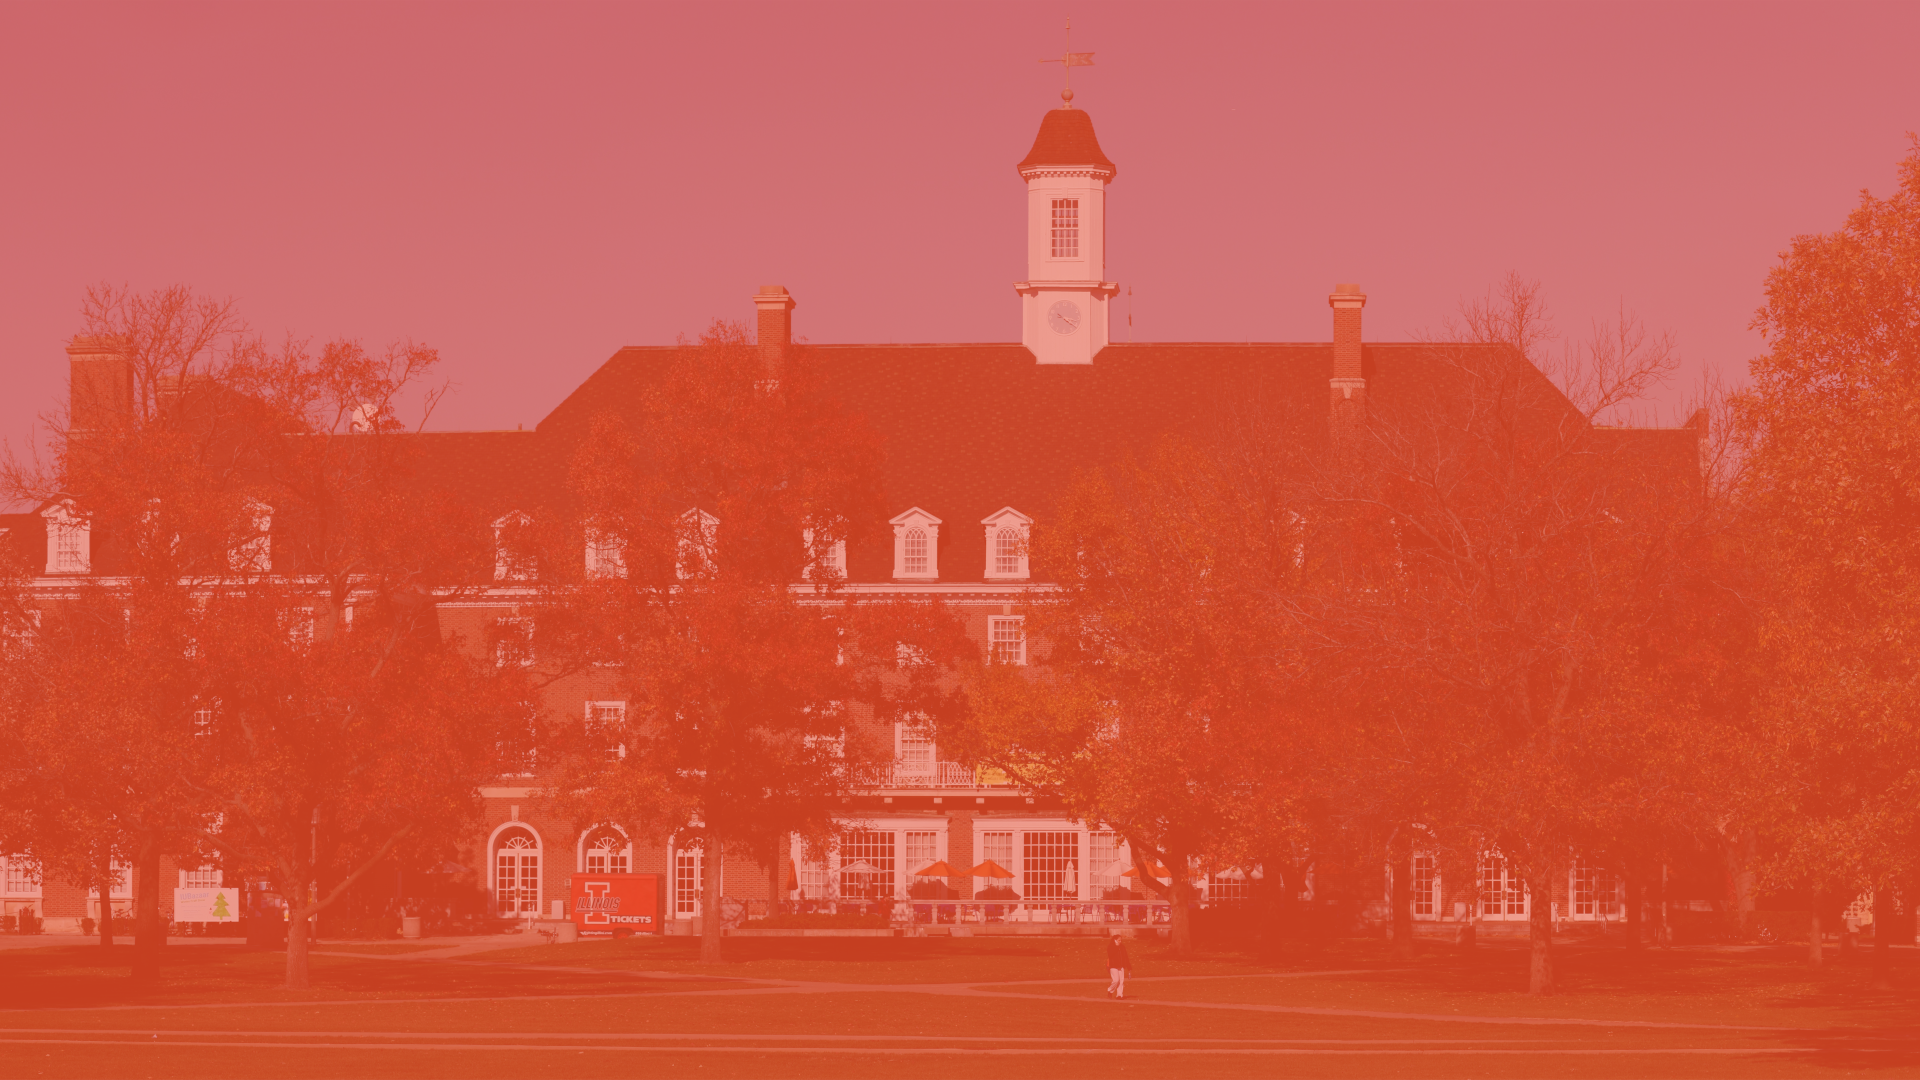
\includegraphics[width=\paperwidth, height=\paperheight]{imgs/uiuc.png}
    \end{textblock*} 
}{}

\begin{document}

\frame{\titlepage}

\section{Introduction}

\begin{frame}
  \frametitle{Background \& Motivations}

  \begin{figure}
      \centering
      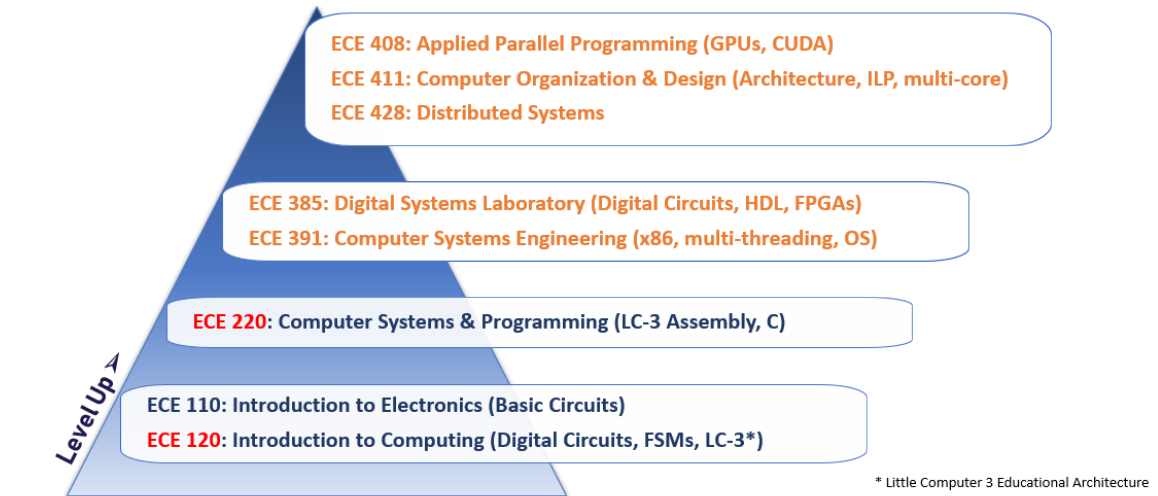
\includegraphics[width=250px]{courses.png}
  \end{figure}
  \vfill
  \begin{itemize}
    \item \textbf{ECE 120:} An introductory Electrical and Computer Engineering course at UIUC with $\sim$400 students each semester.
    \item \textbf{Goal:} Introduce students to concepts in parallel computing early on to present a more realistic view on computing and spark interest for related higher level courses
    %\item 
  \end{itemize}
\end{frame}

\begin{frame}
    \frametitle{Extra Credit Setup}

    \begin{figure}[htbp]
      \centering
      \begin{subfigure}[b]{0.45\textwidth}
        \centering
        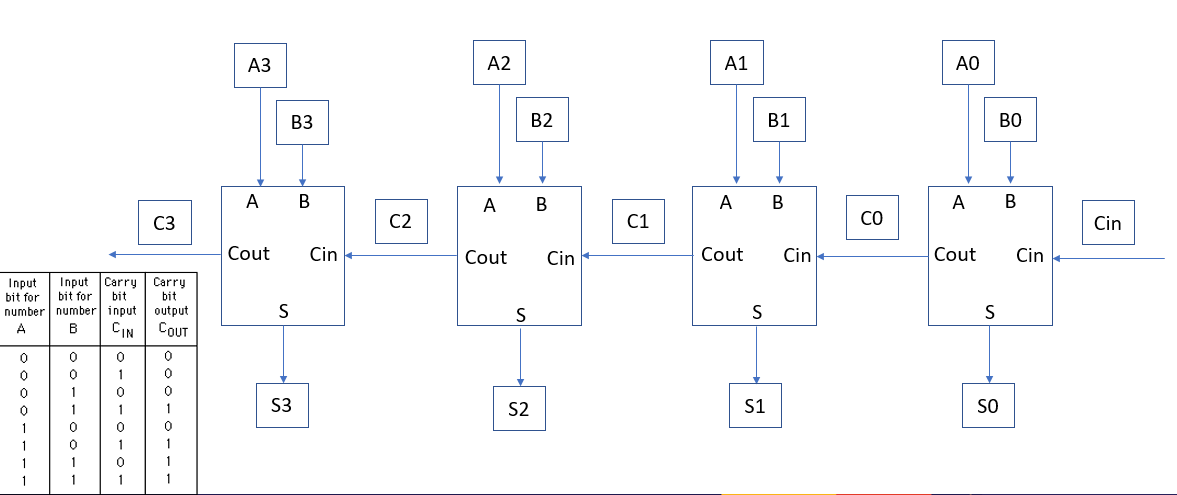
\includegraphics[width=\linewidth]{parallel_add.png}
        \caption{Parallel Adder}
        \label{fig:subfig1}
      \end{subfigure}
      \hfill
      \begin{subfigure}[b]{0.45\textwidth}
        \centering
        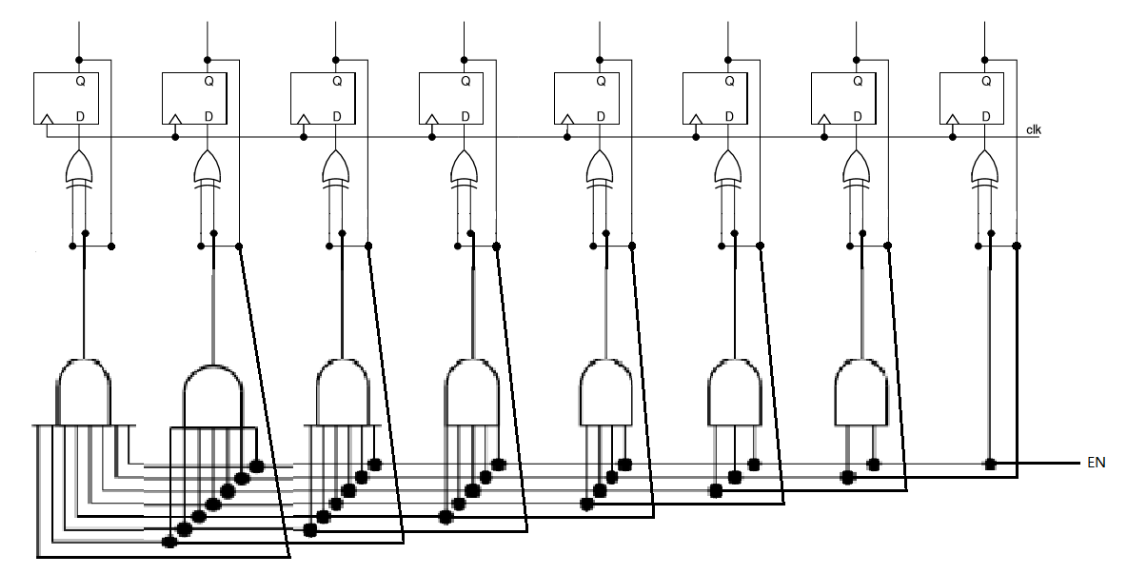
\includegraphics[width=\linewidth]{parallel_counter.png}
        \caption{Parallel Counter}
        \label{fig:subfig2}
      \end{subfigure}
    \end{figure}

    \begin{itemize}
        \item Modules that extended serial counters and adders were developed.
        \item Students were presented with modules of videos and slides.
        \item Extra credit (1.5\% applied to homework) was given for completing a related retention quiz.
    \end{itemize}
     
\end{frame}

\begin{frame}
    \frametitle{Prior Work}

    \begin{itemize}
      \item Prior work has indicated the extra credit has a high participation rate and students perform well. \\ \vspace{0.25cm}
      \item This leaves a gap in our qualitative understanding of these modules and their impacts. \\ \vspace{0.25cm}
      \item \textbf{Goal:} Complete the picture to determine the impact of introducing these concepts as extra-credit modules on students.
    \end{itemize}
\end{frame}


\begin{frame}
    \frametitle{Analysis}

    \begin{minipage}{0.45\textwidth}
      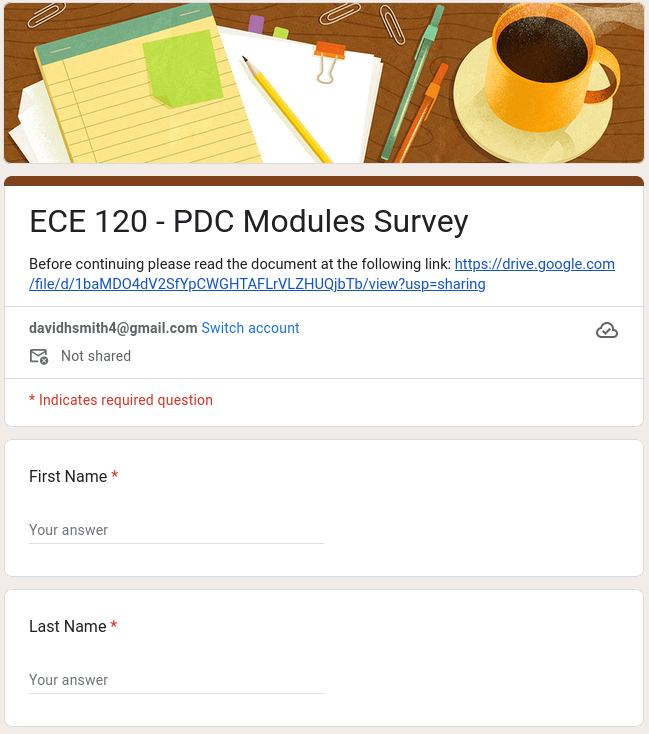
\includegraphics[width=\textwidth]{survey.png}
    \end{minipage}
    \begin{minipage}{0.54\textwidth}
      \begin{itemize}
        \item We created a survey for both students who completed and those did not complete the extra credit modules. 
        \item Each contained a mix of 5 point Likert scale and short response questions.
        \item Received 105 responses between two semesters.
      \end{itemize}
    \end{minipage}
    
    % Make a minipage

\end{frame}

\begin{frame}[fragile]
    \frametitle{Framing the Results}

    \begin{minipage}{0.45\textwidth}
      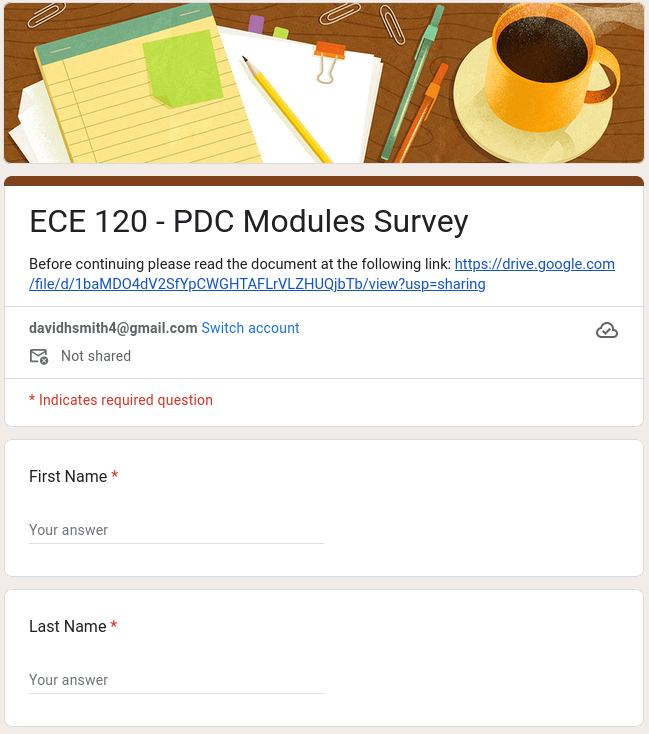
\includegraphics[width=\textwidth]{survey.png}
    \end{minipage}
    \begin{minipage}{0.54\textwidth}
        \begin{itemize}
            \item The survey questions covered the following topics:
            \begin{itemize}
                \item Motivations
                \item Anxiety
                \item Learning and Interest
            \end{itemize}
            \item Responses to short response questions were inductively coded and grouped into themes.
        \end{itemize}
    \end{minipage}

\end{frame}


\section{Motivations}


\begin{frame}[fragile]
    \frametitle{Motivations for Completing the Extra Credit}

    \begin{itemize}
      \item \textbf{Personal Edification:}\\
        \begin{quote}
          ``I thought that it would've been a good opportunity to learn more about
          the topics I've learned during the class''
        \end{quote}
      \item \textbf{Approachability:}\\
        \begin{quote}
          ``The extra credit did not seem like it would take too much time and it seemed simple.''
        \end{quote}
      \item \textbf{Maximizing Grades:}\\
        \begin{quote}
          ``Extra-credit assignments are a great way of improving grades for
          students who might've fallen behind. Each course should have a
          substantiated amount of them to help struggling students succeed.''
        \end{quote}
    \end{itemize}

\end{frame}

\begin{frame}
    \frametitle{Potential Motivators for Those Who Did Not}

    \begin{itemize}
      \item \textbf{Insufficient Grade:}\\
        \begin{quote}
          ``If my [homework] grade was worse I would have been motivated to focus on it''
        \end{quote}
      \item \textbf{Changing Category:}\\
        \begin{quote}
          ``Potentially adding credit to a category like exams instead.''
        \end{quote}
      \item \textbf{Removing Caps:}\\
        \begin{quote}
          ``if the extra credit could allow the grade to go beyond their percentage caps.''
        \end{quote}
    \end{itemize}


\end{frame}


\section{Anxiety}

\begin{frame}
    \frametitle{Relationship Between Extra Credit Opportunities and Anxiety}

    \begin{figure}
      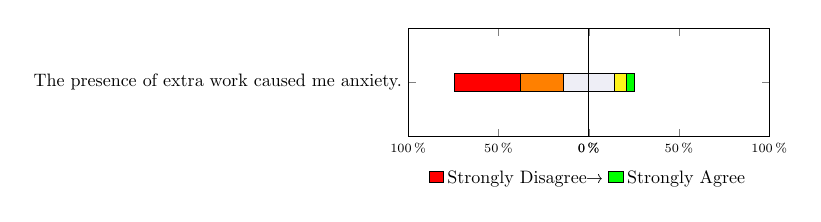
\begin{tikzpicture}[scale=0.65]
    \pgfplotstableread{
Semester 1        2          3           4          5         
Q1       36.61971 23.94366   28.169014   7.042253   4.225352  
    }\frequency
    \begin{axis}[
        scale only axis,
        name=ax1,
        legend cell align=center,
        legend columns=-1,
        legend style={at={(1,-0.25)},anchor=north,draw=none},
        xbar stacked,
        xmin=-100,
        xmax=0,
        try min ticks=3,
        xticklabel style = {font=\scriptsize},
        xticklabel=\pgfmathparse{abs(\tick)}\pgfmathprintnumber{\pgfmathresult}\,$\%$,
        ytick=data,
        yticklabel style={align=left},
        yticklabels={
            The presence of extra work caused me anxiety.,
            Completing the extra credit made me more \\ confident in my ability to succeed in the course.
        },
        enlarge y limits={abs=0.45cm},
        width=100px,
        height=60px
    ]
        \addlegendimage{fill=red}
        \addlegendimage{fill=green}
        \addplot [fill=gray!70!blue!10] table [x expr=-(\thisrow{3}/2), meta=Semester ,y expr=\coordindex] {\frequency};
        \addplot [fill=orange] table [x expr=-\thisrow{2}, meta=Semester ,y expr=\coordindex] {\frequency};
        \addplot [fill=red] table [x expr=-\thisrow{1}, meta=Semester ,y expr=\coordindex] {\frequency};
        \addlegendentry{Strongly Disagree\textrightarrow} 
        \addlegendentry{Strongly Agree}
    \end{axis}

    \begin{axis}[
        scale only axis,
        at=(ax1.south east),
        xbar stacked,
        xmin=0,
        xmax=100,
        xticklabel style = {font=\scriptsize},
        try min ticks=3,
        xticklabel=\pgfmathparse{abs(\tick)}\pgfmathprintnumber{\pgfmathresult}\,$\%$,
        ytick=data,
        yticklabels={},
        enlarge y limits={abs=0.45cm},
        width=100px,
        height=60px
    ]

        \addplot [fill=gray!70!blue!10] table [x expr=(\thisrow{3}/2), meta=Semester ,y expr=\coordindex] {\frequency};
        \addplot [fill=yellow!90] table [x=4, meta=Semester ,y expr=\coordindex] {\frequency};
        \addplot [fill=green] table [x=5, meta=Semester ,y expr=\coordindex] {\frequency};

    \end{axis}
    \vspace{-3mm}
\end{tikzpicture}



    \end{figure}

    \begin{itemize}
      \item \textbf{Anxiety Reducation:}
          ``It's nice to have extra points as a cusion for my grade.''
      \item \textbf{No Impact on Anxiety:}
          ``As it was not required, I was not stressed about completing it and would have been fine without doing it.''
      \item \textbf{Anxiety Increase:}
          ``It seemed as though the work was mandatory in order to protect my grade\ldots''
    \end{itemize}

\end{frame}

\section{Learning \&  Interest}

\begin{frame}
    \frametitle{Impacts on Interest in Parallel Computing}

    \begin{figure}
      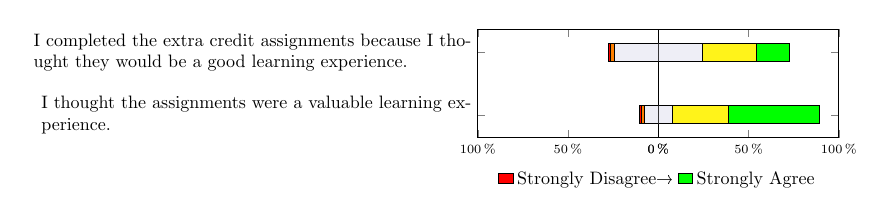
\begin{tikzpicture}[scale=0.65]]
    \pgfplotstableread{
Semester  5    4       3     2        1
Q1        50.70422   30.98591   15.492957   1.408450   1.408450
Q2        18.14516   29.83871   48.991935   2.016129   1.008065
    }\frequency
    \begin{axis}[
        scale only axis,
        name=ax1,
        legend cell align=center,
        legend columns=-1,
        legend style={at={(1,-0.25)},anchor=north,draw=none},
        xbar stacked,
        xmin=-100,
        xmax=0,
        try min ticks=3,
        xticklabel style = {font=\scriptsize},
        xticklabel=\pgfmathparse{abs(\tick)}\pgfmathprintnumber{\pgfmathresult}\,$\%$,
        ytick=data,
        yticklabel style={align=left},
        yticklabels={
            I thought the assignments were a valuable learning 
            ex-\\ perience.,
            I completed the extra credit assignments because I 
            tho- \\ught they would be a good learning experience.
        },
        enlarge y limits={abs=0.45cm},
        width=100px,
        height=60px
    ]
        \addlegendimage{fill=red}
        \addlegendimage{fill=green}
        \addplot [fill=gray!70!blue!10] table [x expr=-(\thisrow{3}/2), meta=Semester ,y expr=\coordindex] {\frequency};
        \addplot [fill=orange] table [x expr=-\thisrow{2}, meta=Semester ,y expr=\coordindex] {\frequency};
        \addplot [fill=red] table [x expr=-\thisrow{1}, meta=Semester ,y expr=\coordindex] {\frequency};
        \addlegendentry{Strongly Disagree\textrightarrow} 
        \addlegendentry{Strongly Agree}
    \end{axis}

    \begin{axis}[
        scale only axis,
        at=(ax1.south east),
        xbar stacked,
        xmin=0,
        xmax=100,
        xticklabel style = {font=\scriptsize},
        try min ticks=3,
        xticklabel=\pgfmathparse{abs(\tick)}\pgfmathprintnumber{\pgfmathresult}\,$\%$,
        ytick=data,
        yticklabels={},
        enlarge y limits={abs=0.45cm},
        width=100px,
        height=60px
    ]

        \addplot [fill=gray!70!blue!10] table [x expr=(\thisrow{3}/2), meta=Semester ,y expr=\coordindex] {\frequency};
        \addplot [fill=yellow!90] table [x=4, meta=Semester ,y expr=\coordindex] {\frequency};
        \addplot [fill=green] table [x=5, meta=Semester ,y expr=\coordindex] {\frequency};

    \end{axis}
    \vspace{-3mm}
\end{tikzpicture}



    \end{figure}
    \vfill
    \begin{quote}
      ``I appreciated the carry look ahead assignment as it had me 
      \textcolor{orange}{\textbf{apply
      patterns that I recognized}} \ldots It felt satisfying seeing how I can
      apply a pattern I recognized.''
    \end{quote}
\end{frame}

\begin{frame}
    \frametitle{Impacts on Interest in Parallel Computing}

    \begin{figure}
      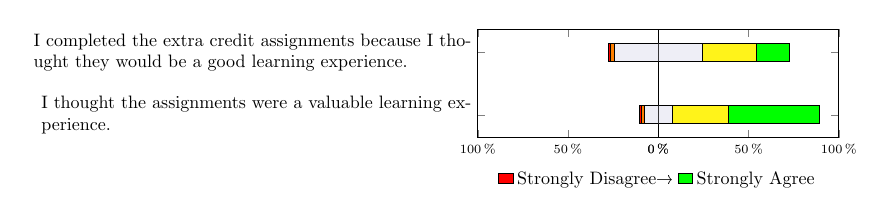
\begin{tikzpicture}[scale=0.65]]
    \pgfplotstableread{
Semester  5    4       3     2        1
Q1        50.70422   30.98591   15.492957   1.408450   1.408450
Q2        18.14516   29.83871   48.991935   2.016129   1.008065
    }\frequency
    \begin{axis}[
        scale only axis,
        name=ax1,
        legend cell align=center,
        legend columns=-1,
        legend style={at={(1,-0.25)},anchor=north,draw=none},
        xbar stacked,
        xmin=-100,
        xmax=0,
        try min ticks=3,
        xticklabel style = {font=\scriptsize},
        xticklabel=\pgfmathparse{abs(\tick)}\pgfmathprintnumber{\pgfmathresult}\,$\%$,
        ytick=data,
        yticklabel style={align=left},
        yticklabels={
            I thought the assignments were a valuable learning 
            ex-\\ perience.,
            I completed the extra credit assignments because I 
            tho- \\ught they would be a good learning experience.
        },
        enlarge y limits={abs=0.45cm},
        width=100px,
        height=60px
    ]
        \addlegendimage{fill=red}
        \addlegendimage{fill=green}
        \addplot [fill=gray!70!blue!10] table [x expr=-(\thisrow{3}/2), meta=Semester ,y expr=\coordindex] {\frequency};
        \addplot [fill=orange] table [x expr=-\thisrow{2}, meta=Semester ,y expr=\coordindex] {\frequency};
        \addplot [fill=red] table [x expr=-\thisrow{1}, meta=Semester ,y expr=\coordindex] {\frequency};
        \addlegendentry{Strongly Disagree\textrightarrow} 
        \addlegendentry{Strongly Agree}
    \end{axis}

    \begin{axis}[
        scale only axis,
        at=(ax1.south east),
        xbar stacked,
        xmin=0,
        xmax=100,
        xticklabel style = {font=\scriptsize},
        try min ticks=3,
        xticklabel=\pgfmathparse{abs(\tick)}\pgfmathprintnumber{\pgfmathresult}\,$\%$,
        ytick=data,
        yticklabels={},
        enlarge y limits={abs=0.45cm},
        width=100px,
        height=60px
    ]

        \addplot [fill=gray!70!blue!10] table [x expr=(\thisrow{3}/2), meta=Semester ,y expr=\coordindex] {\frequency};
        \addplot [fill=yellow!90] table [x=4, meta=Semester ,y expr=\coordindex] {\frequency};
        \addplot [fill=green] table [x=5, meta=Semester ,y expr=\coordindex] {\frequency};

    \end{axis}
    \vspace{-3mm}
\end{tikzpicture}



    \end{figure}
    \vfill
    \begin{quote}
      ``Just enough info to catch my attention, not quite enough to satisfy my
      curiosity. \textcolor{orange}{\textbf{The assignments gave meaning to parallel computing courses,
      instead of them being just other options from the list.}}''
    \end{quote}
    \vfill
\end{frame}

\begin{frame}
    \frametitle{Impacts on Interest in Parallel Computing}

    \begin{figure}
      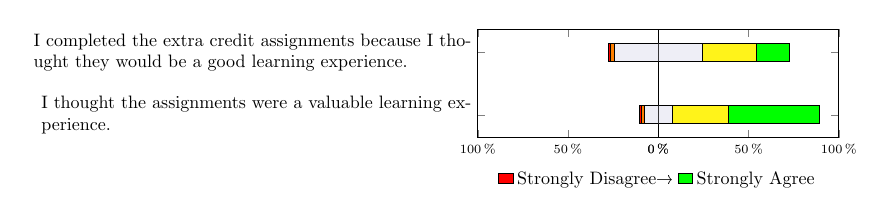
\begin{tikzpicture}[scale=0.65]]
    \pgfplotstableread{
Semester  5    4       3     2        1
Q1        50.70422   30.98591   15.492957   1.408450   1.408450
Q2        18.14516   29.83871   48.991935   2.016129   1.008065
    }\frequency
    \begin{axis}[
        scale only axis,
        name=ax1,
        legend cell align=center,
        legend columns=-1,
        legend style={at={(1,-0.25)},anchor=north,draw=none},
        xbar stacked,
        xmin=-100,
        xmax=0,
        try min ticks=3,
        xticklabel style = {font=\scriptsize},
        xticklabel=\pgfmathparse{abs(\tick)}\pgfmathprintnumber{\pgfmathresult}\,$\%$,
        ytick=data,
        yticklabel style={align=left},
        yticklabels={
            I thought the assignments were a valuable learning 
            ex-\\ perience.,
            I completed the extra credit assignments because I 
            tho- \\ught they would be a good learning experience.
        },
        enlarge y limits={abs=0.45cm},
        width=100px,
        height=60px
    ]
        \addlegendimage{fill=red}
        \addlegendimage{fill=green}
        \addplot [fill=gray!70!blue!10] table [x expr=-(\thisrow{3}/2), meta=Semester ,y expr=\coordindex] {\frequency};
        \addplot [fill=orange] table [x expr=-\thisrow{2}, meta=Semester ,y expr=\coordindex] {\frequency};
        \addplot [fill=red] table [x expr=-\thisrow{1}, meta=Semester ,y expr=\coordindex] {\frequency};
        \addlegendentry{Strongly Disagree\textrightarrow} 
        \addlegendentry{Strongly Agree}
    \end{axis}

    \begin{axis}[
        scale only axis,
        at=(ax1.south east),
        xbar stacked,
        xmin=0,
        xmax=100,
        xticklabel style = {font=\scriptsize},
        try min ticks=3,
        xticklabel=\pgfmathparse{abs(\tick)}\pgfmathprintnumber{\pgfmathresult}\,$\%$,
        ytick=data,
        yticklabels={},
        enlarge y limits={abs=0.45cm},
        width=100px,
        height=60px
    ]

        \addplot [fill=gray!70!blue!10] table [x expr=(\thisrow{3}/2), meta=Semester ,y expr=\coordindex] {\frequency};
        \addplot [fill=yellow!90] table [x=4, meta=Semester ,y expr=\coordindex] {\frequency};
        \addplot [fill=green] table [x=5, meta=Semester ,y expr=\coordindex] {\frequency};

    \end{axis}
    \vspace{-3mm}
\end{tikzpicture}



    \end{figure}

    \vfill
    \begin{itemize}
        \item ``It did not really change my interest in the parallel computing topic.'' \\ \vspace{0.25cm} 
        \item ``I wasn't too interested in the topic to begin with, \textcolor{orange}{\textbf{so I just did the assignment for the points.}}''\\ \vspace{0.25cm}
        \item ``\textcolor{orange}{\textbf{I am already interested in power electronics and electrical propulsion}}, so doing these extra credit quizzes isn't enough for me to change my area of interest.''
    \end{itemize}

\end{frame}

\section{Takeaways}

\begin{frame}
    \frametitle{Key Takeaways}

    \begin{itemize}
      \item Students had a positive, or at worst neutral, response to the concepts introduced in the extra credit modules.
      \item There appear to be additional benefits to introducing them as extra credit (e.g., anxiety reduction).
      \item Modules such as these appear to be a useful vector to introduce higher level concepts early on.
      \item For details on the modules and their implementation please contact \textcolor{blue}{ubhowmik@illinois.edu}
    \end{itemize}
    \vfill
      \begin{centered}
          \textbf{\Large Thank you!}
      \end{centered}
\end{frame}


\end{document}
